\begin{activity} \label{A:3.3.1}  Let $g(x) = \frac{1}{3}x^3 - 2x + 2.$
	\ba
	\item Find all critical values of $g$ that lie in the interval $-2 \le x \le 3$.
	\item Use a graphing utility to construct the graph of $g$ on the interval $-2 \le x \le 3$.
	\item From the graph, determine the $x$-values at which the absolute minimum and absolute maximum of $g$ occur on the interval $[-2,3]$.
	\item How do your answers change if we instead consider the interval $-2 \le x \le 2$?
	\item What if we instead consider the interval $-2 \le x \le 1$?
	\ea
\end{activity}
\begin{smallhint}
	\ba
	\item Check that each critical value you find satisfies $-2 \le x \le 3$.
	\item \href{http://wolframalpha.com}{\texttt{http://wolframalfpha.com}} is a great choice.
	\item On the graph, look for the lowest and highest possible values of the function.
	\item Ask yourself the same questions as (a)-(c), simply using the new interval.
	\ea
\end{smallhint}
\begin{bighint}
	\ba
	\item Check that each critical value you find satisfies $-2 \le x \le 3$.
	\item \href{http://wolframalpha.com}{\texttt{http://wolframalfpha.com}} is a great choice.
	\item On the graph, look for the lowest and highest possible values of the function.
	\item Ask yourself the same questions as (a)-(c), simply using the new interval.
	\ea
\end{bighint}
\begin{activitySolution}
	\ba
	\item Since $g'(x) = x^2 - 2$, the critical values of $g$ are $x = \pm \sqrt{2} \approx \pm 1.414$, both of which lie in the interval $-2 \le x \le 3$.
	\item The figure shown below shows three related plots, each with the emphases on the interval provided in (c), (d), and (e).
	\begin{center}
	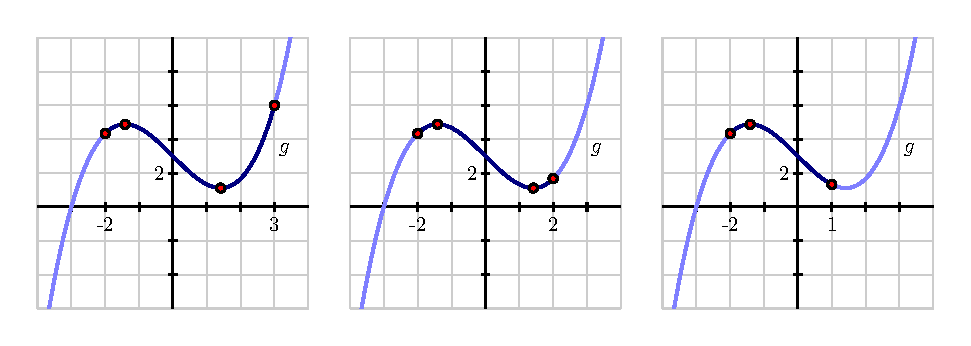
\includegraphics{figures/3_3_Act1Soln.eps}
	\end{center}
	\item On $[-2,3]$, $g$ has a global maximum at $x = 3$ and a global minimum at $x = \sqrt{2}$.
	\item On $[-2,2]$, $g$ has a global maximum at $x = -\sqrt{2}$ and a global minimum at $x = \sqrt{2}$.
	\item On $[-2,3]$, $g$ has a global maximum at $x = -\sqrt{2}$ and a global minimum at $x = 1$.
	\ea
\end{activitySolution}
\aftera